\section{Vendor instructions}
\subsection{Orders view}
By clicking on the \textit{Orders} button in the header, the vendor reaches the orders page, where he can view all the orders placed by customers.
\newline
From this page the vendor can view for each order:
\begin{itemize}
    \item the order code;
    \item the status of the order;
    \item the total and subtotal price;
    \item the quantity of ordered items;
    \item the checkout date;
    \item the username of the customer who placed the order.
\end{itemize}
\begin{figure}[!ht]
    \caption{Orders page viewed from the vendor}
    \vspace{5px}
    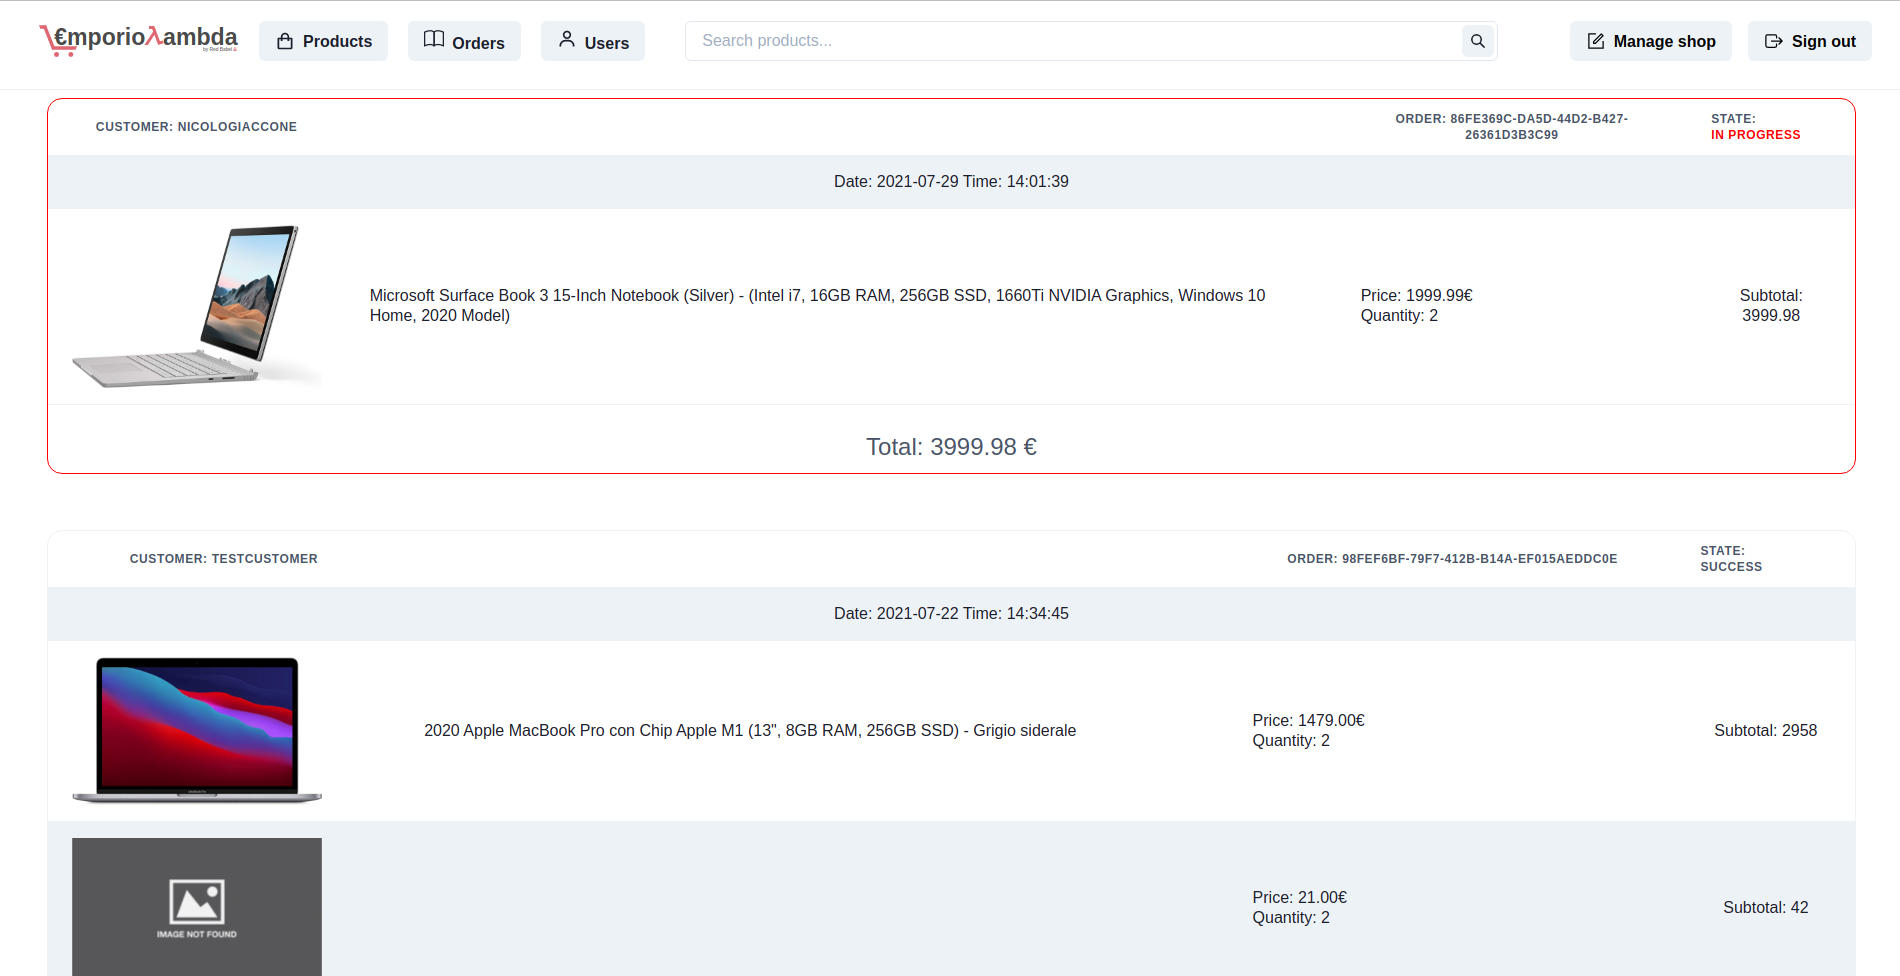
\includegraphics[scale=0.25]{../../../../Images/userManual/ordersVendor.png}
    \centering
\end{figure}
\pagebreak
\subsection{Shop management}
By clicking on the \textit{Manage shop} button in the header, the vendor reaches the page to manage the shop, where he can create a new product, create a new category or delete a category.
\subsubsection{Create new product}
By clicking on \textit{Create New Product}, a screen will be displayed where the vendor can insert a new product in the system. Here the vendor can:
\begin{itemize}
    \item enter the product title;
    \item enter the price of the product;
    \item enter the description;
    \item enter the discount;
    \item enter the availability;
    \item insert an image of the product;
    \item select the product category;
    \item add notes.
\end{itemize}
Product's title, price, image, availability and category are mandatory, if the vendor doesn't fill that a pop-up error appers and the creation is blocked.
After having entered the necessary data for the new product, it will be possible to insert the product by clicking on the \textit{Submit} button at the bottom of the page.
\begin{figure}[!ht]
    \caption{Create new product section viewed from the vendor}
    \vspace{5px}
    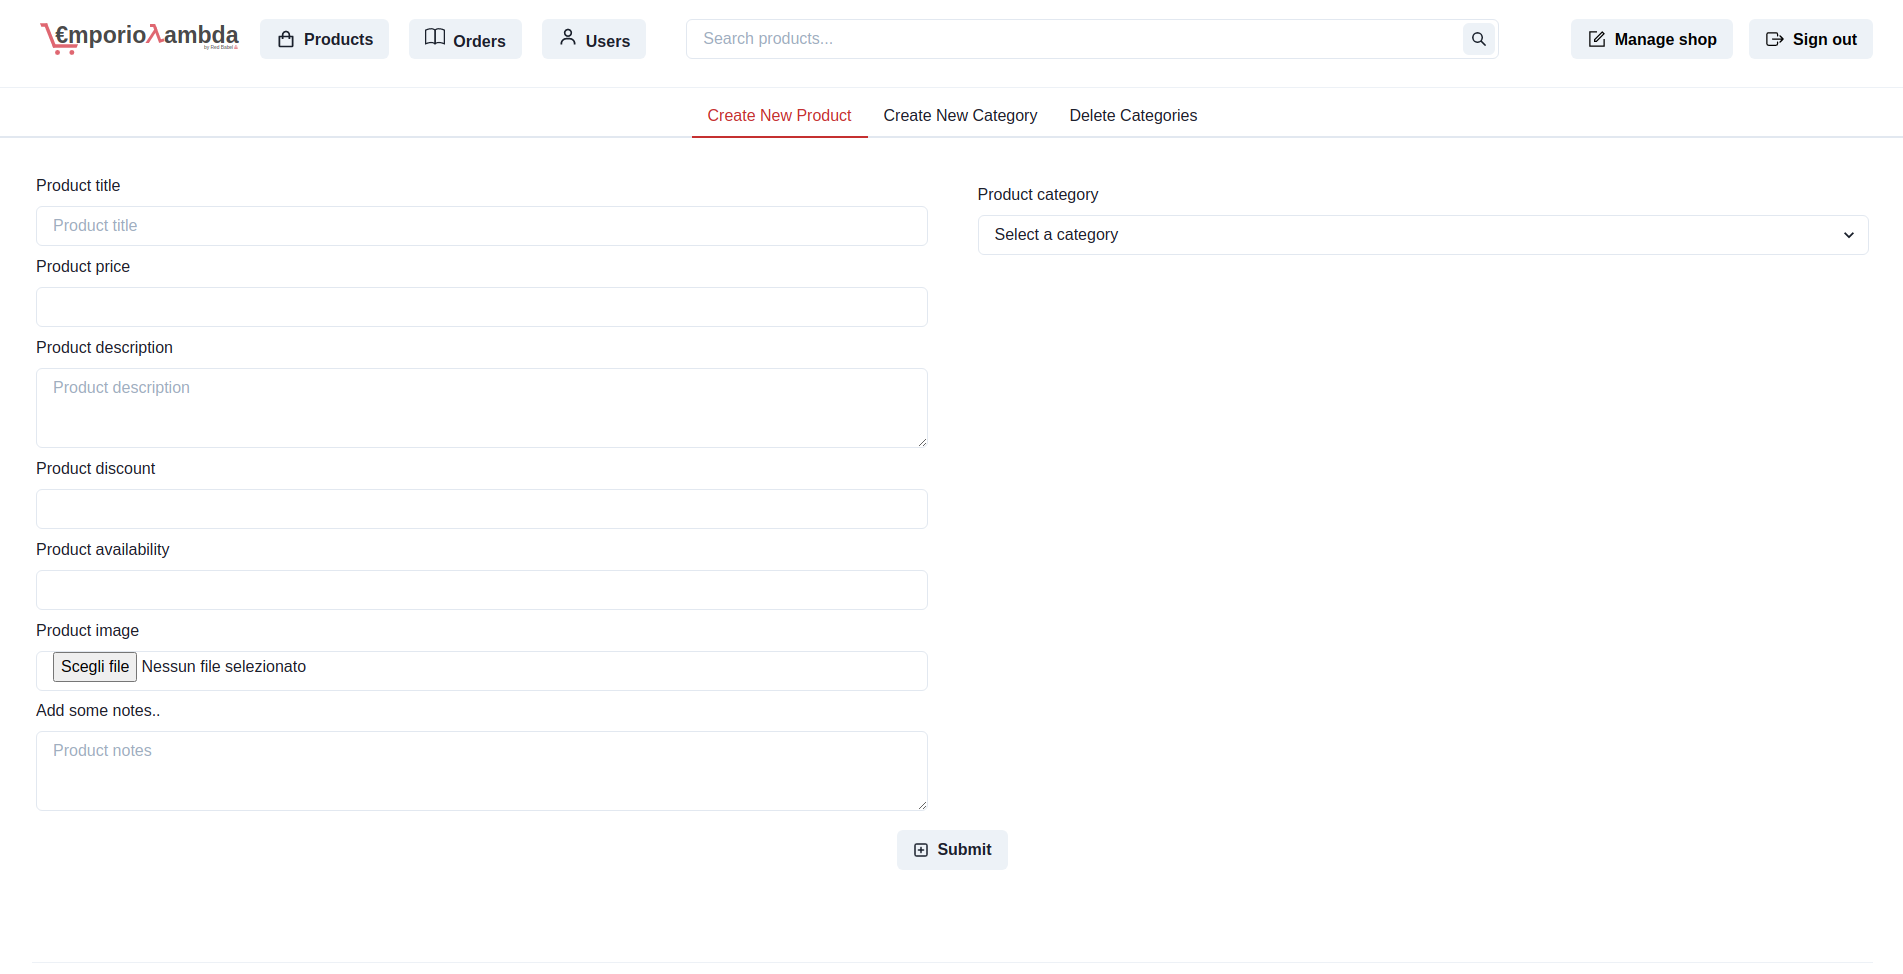
\includegraphics[scale=0.25]{../../../../Images/userManual/createNewProductVendor.png}
    \centering
\end{figure}
\pagebreak
\subsubsection{Create new category}
By clicking on \textit{Create New Category}, a screen will be displayed where the vendor can insert a new category of products in the system. Here the vendor can:
\begin{itemize}
    \item enter the category name;
    \item enter the description;
    \item enter the taxation for the category;
    \item add additional customizable specifications based on the category.
\end{itemize}
After entering the necessary data for the new category, it will be possible to insert the category by clicking on the \textit{Submit} button at the bottom of the page.
\begin{figure}[!ht]
    \caption{Create new category section viewed from the vendor}
    \vspace{5px}
    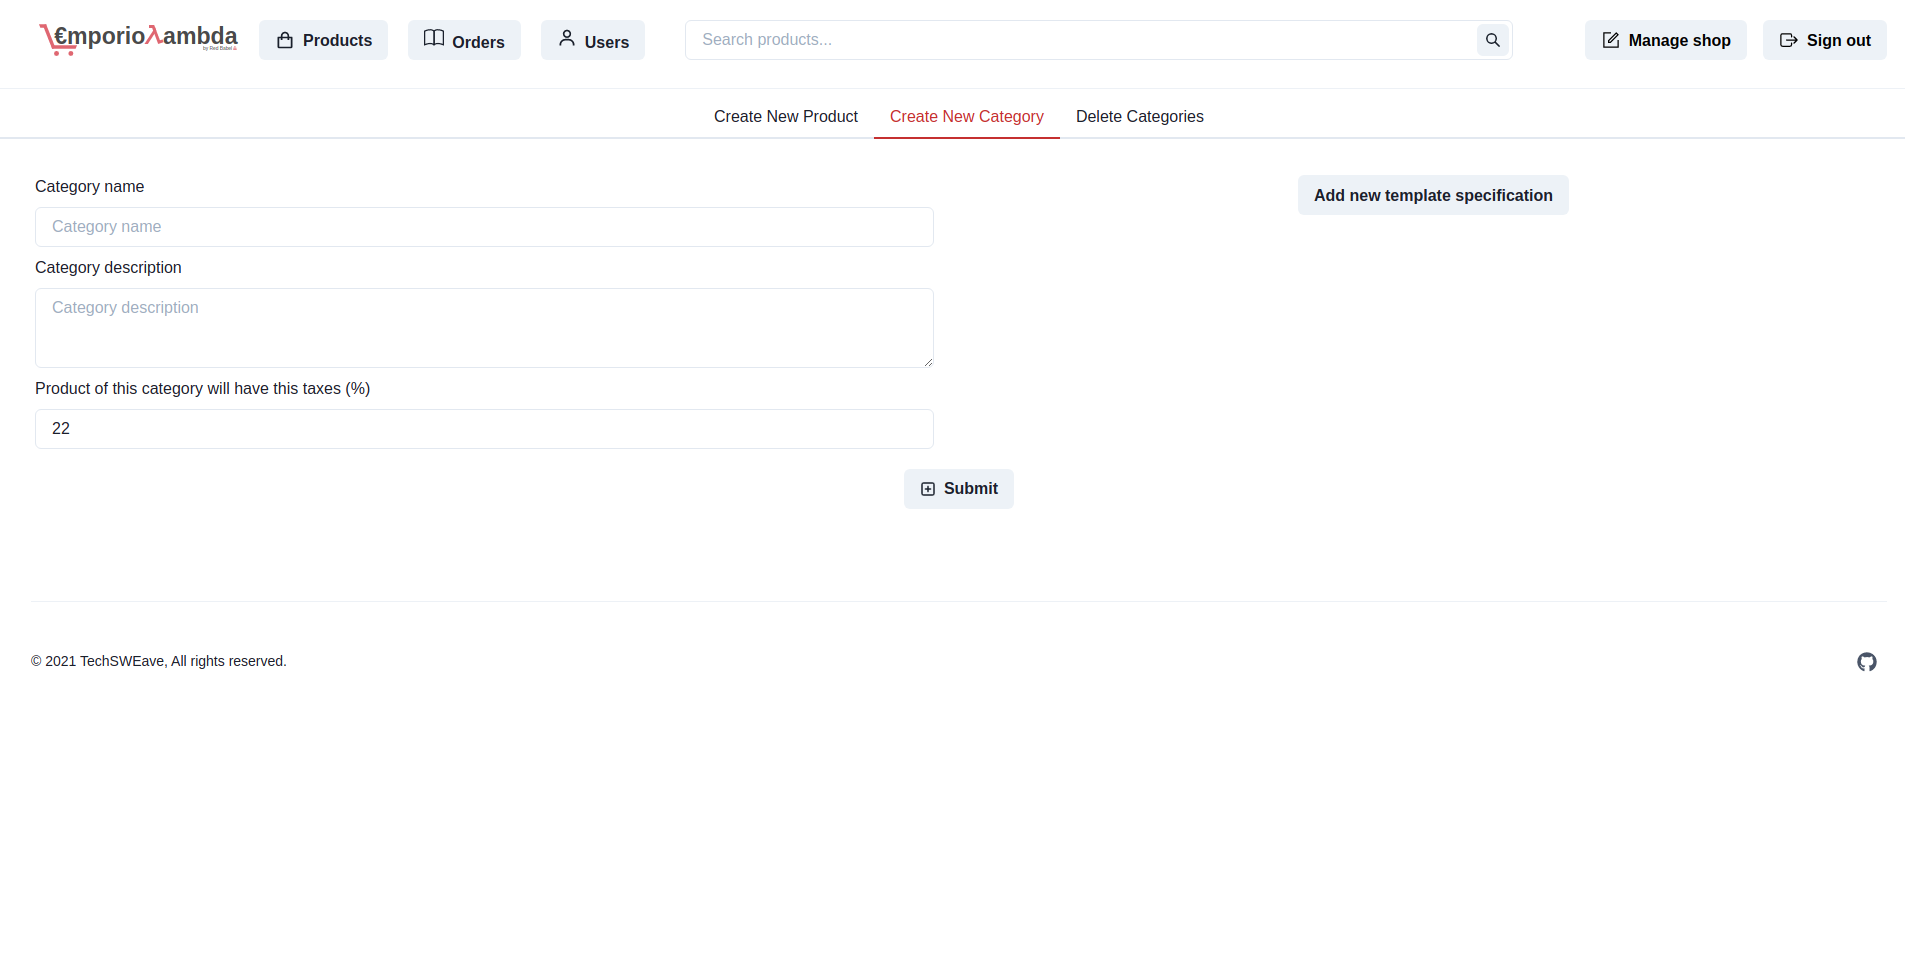
\includegraphics[scale=0.25]{../../../../Images/userManual/createNewCategoryVendor.png}
    \centering
\end{figure}
\subsubsubsection{Add new template specification}
By clicking on the \textit{Add New Template Specification} button displayed at the top right of the screen for adding a new category, the vendor can add one or more additional customizable specifications related to the category.
\linebreak
A row will be displayed for each new specification, in which the vendor can enter:
\begin{itemize}
    \item the name of the specification;
    \item the unit of measurement of the specification.
\end{itemize}
The specifications will finally be added to the category by clicking on the \textit{Submit} button to create the category itself.
\begin{figure}[!ht]
    \caption{Create new category section viewed from the vendor}
    \vspace{5px}
    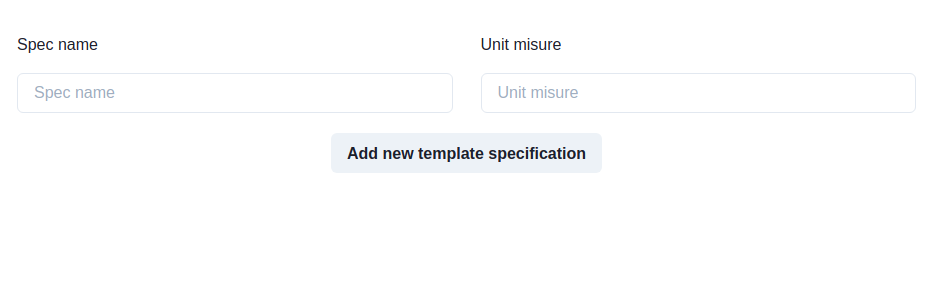
\includegraphics[scale=0.25]{../../../../Images/userManual/addSpecificationCategoryVendor.png}
    \centering
\end{figure}
\pagebreak
\subsubsection{Delete categories}
By clicking on \textit{Delete Categories}, a screen will be displayed where the vendor can delete the categories.\linebreak
To remove a specific category the vendor will have to click on the button \textit{DELETE CATEGORY}, displayed on the bottom of the category that he wants to delete.
\begin{figure}[!ht]
    \caption{Delete categories section viewed from the vendor}
    \vspace{5px}
    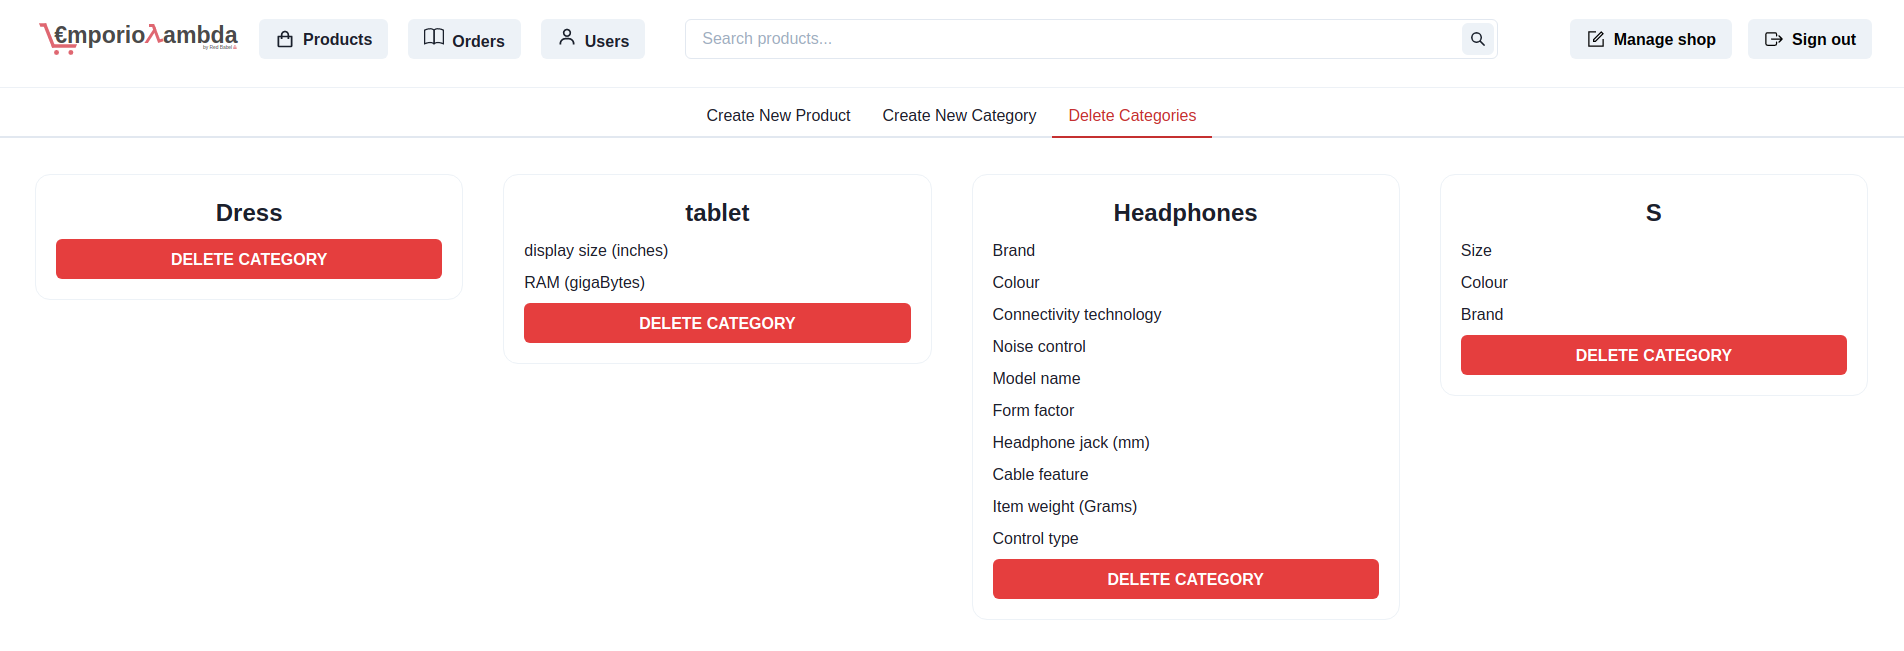
\includegraphics[scale=0.25]{../../../../Images/userManual/deleteCategoriesVendor.png}
    \centering
\end{figure}
\pagebreak
\subsection{Users view}
By clicking on the \textit{Users} button in the header, the vendor reaches the screen to view all registered users on the site.
Here the vendor can view for each user:
\begin{itemize}
    \item the username;
    \item name and surname;
    \item the date of birth;
    \item the address.
\end{itemize}
The vendor can also send an email to the user by clicking directly on the email of the user.
\begin{figure}[!ht]
    \caption{Users page viewed from the vendor}
    \vspace{5px}
    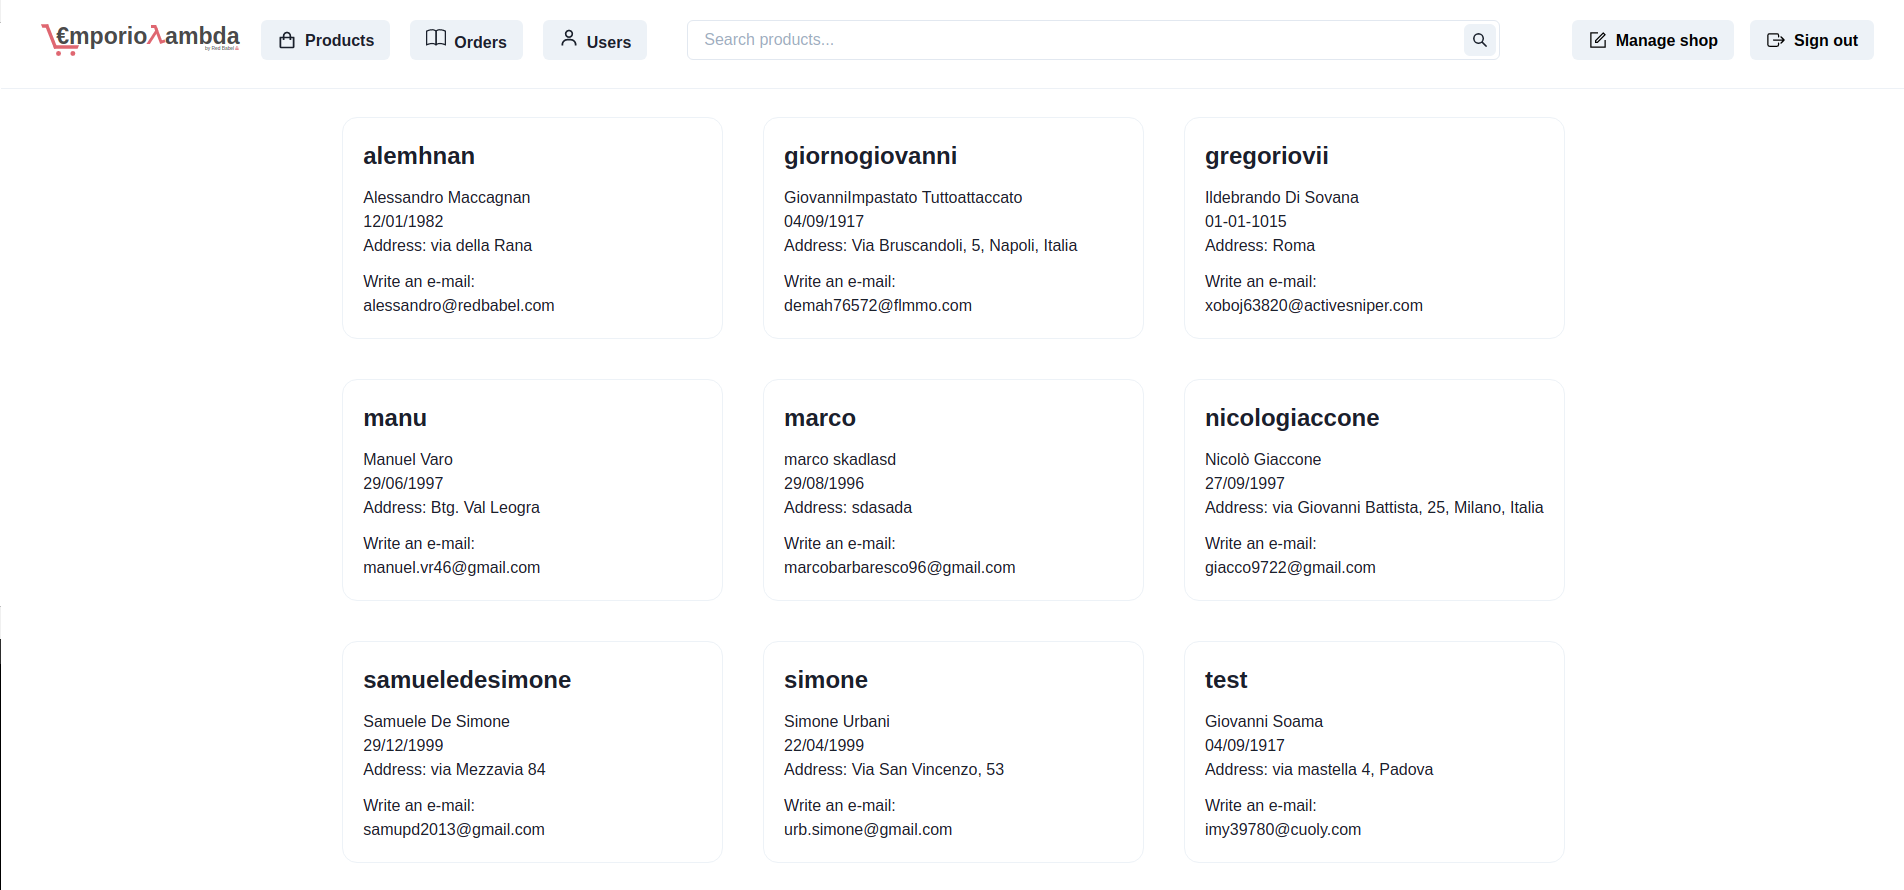
\includegraphics[scale=0.25]{../../../../Images/userManual/usersVendor.png}
    \centering
\end{figure}
\pagebreak
\subsection{Products view}
By clicking on the \textit{Products} button displayed in the top left of the header, the vendor will reach the page from which he can view a list of all the products for sale on the site, both salable and private.
Here the vendor can view for each product:
\begin{itemize}
    \item the image;
    \item the price;
    \item the name.
\end{itemize}
\begin{figure}[!ht]
    \caption{Products page viewed from the vendor}
    \vspace{5px}
    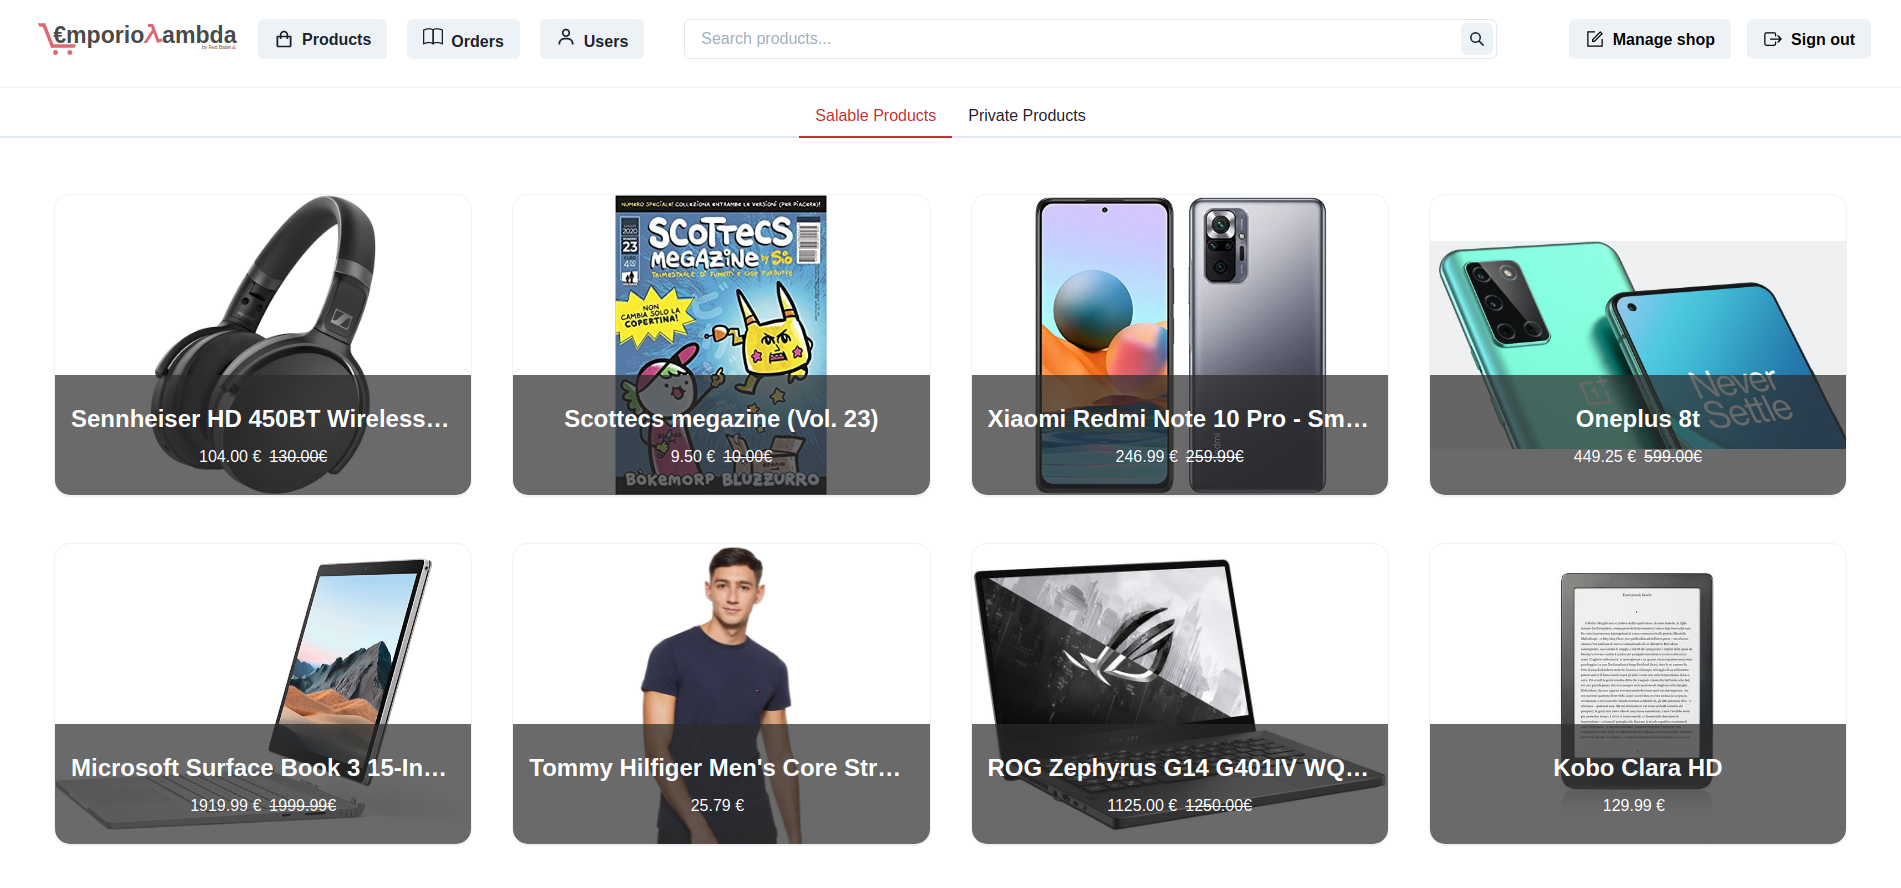
\includegraphics[scale=0.25]{../../../../Images/userManual/productsVendor.png}
    \centering
\end{figure}
\pagebreak
\subsubsection{Product detail}
By clicking on the image of a single product in the products page, the vendor will be redirected to the product detail page, where it will be possible to view all the characteristics of the product and its details.
\begin{figure}[!ht]
    \caption{Product detail page viewed from the vendor}
    \vspace{5px}
    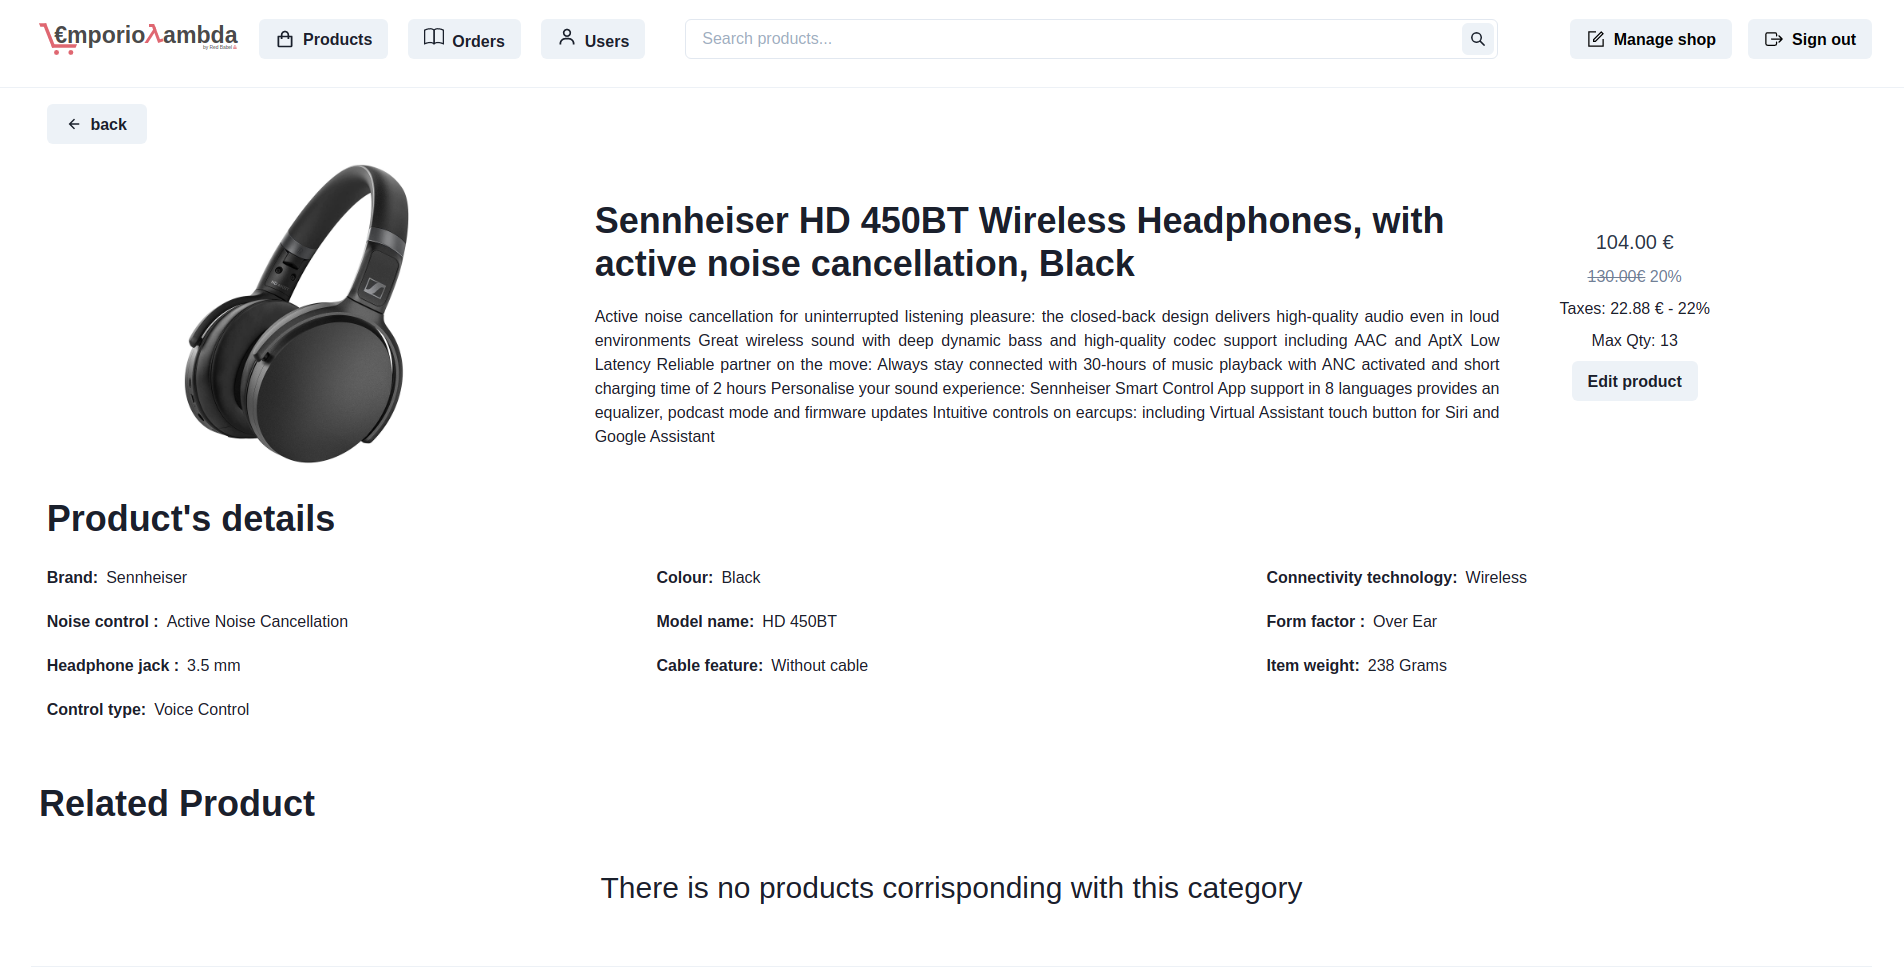
\includegraphics[scale=0.25]{../../../../Images/userManual/productDetailVendor.png}
    \centering
\end{figure}
\pagebreak
\subsubsection{Edit product}
By opening a product the vendor will be redirected to the screen where he can edit all the product details. After possibly changing the data, the vendor can save the changes by clicking on the \textit{Submit} button or clicking the \textit{View Product} the vendor could see the PDP page. From this screen it is also possible to delete the product by clicking on the \textit{DELETE PRODUCT} button.
\begin{figure}[!ht]
    \caption{Edit product page viewed from the vendor}
    \vspace{5px}
    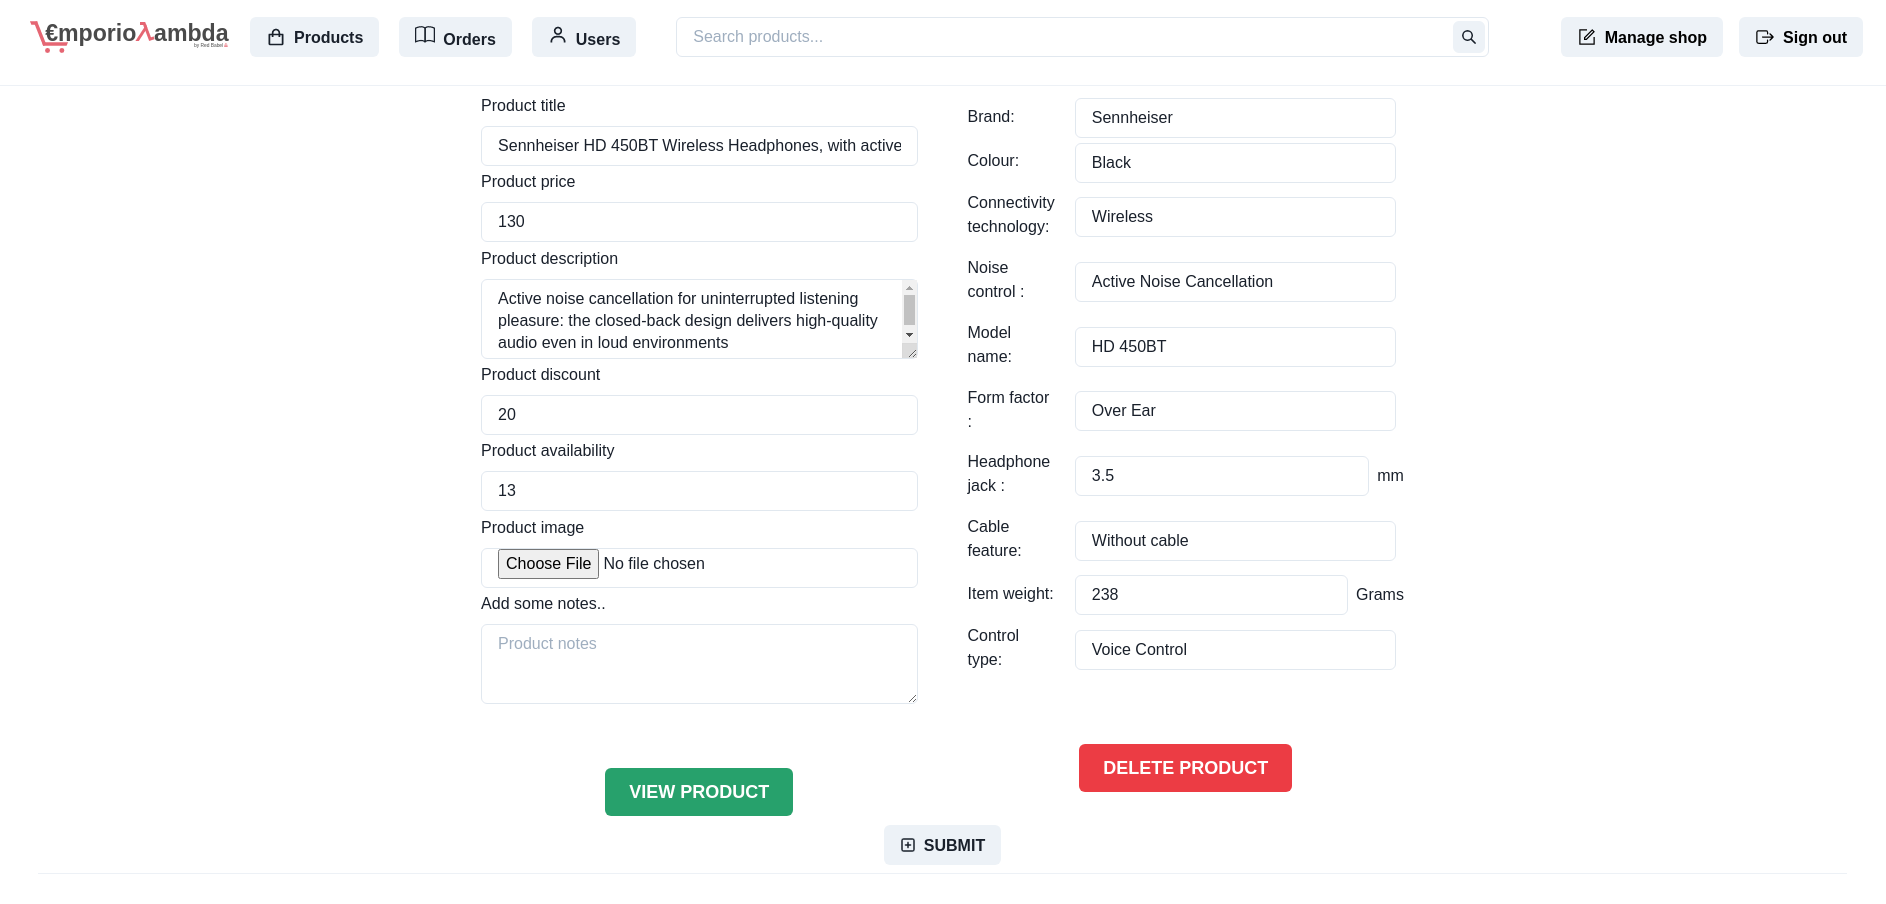
\includegraphics[scale=0.25]{../../../../Images/userManual/editProductVendor.png}
    \centering
\end{figure}
